\documentclass[man,12pt,floatsintext]{apa7}

% =========================================================
% Idioma y fuentes
% =========================================================
\usepackage[spanish,es-tabla]{babel}
\usepackage{fontspec}

\setmainfont{IBM Plex Serif}
\setsansfont{IBM Plex Sans}
\setmonofont{IBM Plex Mono}

% =========================================================
% Paquetes
% =========================================================
\usepackage{csquotes}
\usepackage{graphicx}
\usepackage{float}
\usepackage{booktabs}
\usepackage{longtable}
\usepackage{array}
\usepackage{tabularx}
\usepackage{ragged2e}
\usepackage{pdflscape}
\usepackage{listings}
\usepackage{hyperref}
\usepackage{xurl}

% Corrige warning de fancyhdr en apa7
\setlength{\headheight}{16pt}

% Mejora cortes de línea en tablas con rutas, scripts y texto técnico
\setlength{\emergencystretch}{3em}
\newcolumntype{L}[1]{>{\RaggedRight\arraybackslash}p{#1}}
\newcolumntype{Y}{>{\RaggedRight\arraybackslash}X}

% =========================================================
% Bibliografía APA 7
% =========================================================
\usepackage[
  backend=biber,
  style=apa,
  sorting=nyt
]{biblatex}

\addbibresource{referencias.bib}

% =========================================================
% Metadatos mínimos requeridos por apa7
% =========================================================
\title{Diseño, transformación e implementación de una base de datos en Oracle 19c para la gestión odontológica}
\shorttitle{Base de datos Oracle 19c para gestión odontológica}
\leftheader{Ávila, Peñaranda y Limachi}

% =========================================================
% Rutas de imágenes
% =========================================================
\graphicspath{
  {figuras/}
  {../01_conceptual_chen/}
  {../03_crows_foot/}
  {../06_evidencias/}
}

% =========================================================
% Configuración de código
% =========================================================
\lstset{
  basicstyle=\ttfamily\footnotesize,
  breaklines=true,
  breakatwhitespace=false,
  frame=single,
  columns=fullflexible,
  keepspaces=true,
  showstringspaces=false,
  tabsize=2
}

% =========================================================
% Comandos de figuras
% =========================================================
\newcommand{\figuranormal}[3]{%
\begin{figure}[H]
\centering
\includegraphics[width=\textwidth,height=0.78\textheight,keepaspectratio]{#1}
\caption{#2}
\label{#3}
\end{figure}
}

\newcommand{\figuraapaisada}[3]{%
\clearpage
\begin{landscape}
\begin{figure}[H]
\centering
\includegraphics[width=0.95\linewidth,height=0.82\textheight,keepaspectratio]{#1}
\caption{#2}
\label{#3}
\end{figure}
\end{landscape}
\clearpage
}

% =========================================================
% Documento
% =========================================================
\begin{document}
\nocite{*}

\thispagestyle{empty}
\begin{center}
  {\Large Universidad Mayor Real y Pontificia de San Francisco\\
    Xavier de Chuquisaca\par}

  \vspace{0.5cm}
  {\large Facultad de Ciencias y Tecnología\par}
  {\large Ingeniería en Ciencias de la Computación\par}

  \vspace{1.2cm}
  {\large SIS306 - Examen Final\par}
  {\large SIS306 - Bases de Datos III\par}

  \vspace{1.2cm}
  {\large Docente: Ing. Edgar T. Espinoza Rodríguez\par}

  \vspace{1.2cm}
  {\large Estudiantes:\par}
  {\large Ávila Serrano Christian Ángel\par}
  {\large Peñaranda Villarroel Hernán Isaac\par}
  {\large Limachi Villarroel Alan Nicolás\par}

  \vspace{1.2cm}
  {\large Fecha de entrega: Martes, 23 de junio de 2026\par}

  \vfill
  {\large Diseño, transformación e implementación de una base de datos en Oracle 19c para la gestión odontológica\par}
\end{center}

\clearpage
\setcounter{page}{1}

\section{Introducción}

El presente informe desarrolla la documentación técnica de una base de datos para la gestión de procesos odontológicos. El dominio considerado incluye registro de pacientes, asignación de carpetas clínicas, programación de citas, atención mediante odontogramas, tratamientos, planes de pago, registro de pagos, compras de suministros e inventario.

El trabajo toma como referencia documental una tesis previa sobre el desarrollo de un sistema de información web para el consultorio odontológico LALYSDENT. En dicha tesis se documenta un sistema web implementado con Laravel, MySQL y arquitectura MVC. A diferencia de esa investigación, el presente informe no se enfoca en el frontend ni en la aplicación web, sino en el diseño, transformación, implementación y validación de la base de datos.

La propuesta fue desarrollada en etapas. Primero, se definieron los requisitos y supuestos del dominio. Luego, se elaboró un modelo conceptual en notación Chen usando diagrams.net. Posteriormente, se realizó la transformación al modelo relacional y se construyó un modelo lógico Crow's Foot en ER/Studio 2003. Finalmente, se implementó el diseño físico en Oracle Database 19c, ejecutado en Docker y administrado mediante DBeaver.

El documento incluye también un diccionario de datos completo, validaciones ejecutadas sobre Oracle 19c y una comparación técnica entre el enfoque MySQL/Laravel documentado en la tesis base y la transformación realizada hacia Oracle 19c.

\section{Objetivos}

\subsection{Objetivo general}

Diseñar, transformar, implementar y validar una base de datos relacional en Oracle Database 19c para la gestión de procesos odontológicos, tomando como referencia documental la tesis del sistema web LALYSDENT desarrollado con Laravel y MySQL.

\subsection{Objetivos específicos}

Identificar las entidades, atributos, relaciones, cardinalidades y restricciones del dominio odontológico documentado en la tesis base.

Elaborar el modelo conceptual en notación Chen usando diagrams.net.

Transformar el modelo conceptual al modelo relacional, definiendo tablas, claves primarias, claves foráneas, restricciones de dominio y relaciones opcionales u obligatorias.

Construir el modelo lógico en notación Crow's Foot mediante ER/Studio 2003.

Implementar el diseño físico en Oracle Database 19c, usando SQL y PL/SQL.

Crear un diccionario de datos completo y contrastarlo con el catálogo técnico de Oracle.

Comparar el enfoque MySQL/Laravel descrito en la tesis base con la transformación realizada hacia Oracle 19c.

Validar la base de datos mediante datos de prueba, consultas de control, triggers y procedimiento almacenado.

\section{Herramientas utilizadas}

\begin{table}[H]
\caption{Herramientas utilizadas en el proyecto}
\centering
\small
\begin{tabularx}{\textwidth}{L{0.28\textwidth}Y}
\toprule
\textbf{Herramienta} & \textbf{Uso en el proyecto} \\
\midrule
diagrams.net / Draw.io & Elaboración del modelo conceptual en notación Chen. \\
ER/Studio 2003 & Elaboración del modelo lógico relacional en notación Crow's Foot. \\
Oracle Database 19c & Motor de base de datos usado para la implementación física. \\
Docker & Ejecución de Oracle 19c en contenedor. \\
DBeaver & Ejecución de scripts SQL/PLSQL y validación de objetos. \\
VSCodium & Edición del proyecto, scripts y documento final. \\
Konsole con zsh & Ejecución de comandos, Git, compilación LaTeX y organización del repositorio. \\
LuaLaTeX + Biber & Compilación del informe final con formato APA 7. \\
Git & Control de versiones del proyecto. \\
\bottomrule
\end{tabularx}
\end{table}

\section{Análisis de requisitos}

\subsection{Materiales del proyecto y fuentes de apoyo}

Para contextualizar el dominio LALYSDENT se consideraron dos materiales principales. El primero fue el sitio web de la tesis base, disponible en \url{https://calvocobos.github.io/}, usado como apoyo documental para comprender los procesos de registro, atención, inventario y finanzas del consultorio odontológico. El segundo fue el repositorio Laravel desarrollado por el equipo del proyecto, disponible en \url{https://github.com/AlanDevPro/sistema-odontologico}, usado para ejecutar y evidenciar la aplicación web propia del sistema \parencite{calvocobos2025web,sistemaodontologicogithub}.

La aplicación Laravel forma parte del trabajo del equipo, pero no reemplaza el objetivo principal del examen. El producto central de este informe sigue siendo el diseño, transformación, implementación y validación de la base de datos Oracle 19c en el schema \texttt{FARMACIAS\_BD3}. Para ejecutar la aplicación web sin alterar dicho diseño, se utilizó un schema separado llamado \texttt{LALYSDENT\_APP}.

\subsection{Alcance funcional tomado de la tesis base}

La tesis base desarrolla un sistema de información web para administrar procesos de registro, atención, inventario y finanzas del consultorio odontológico LALYSDENT. Dicho sistema incluye módulos de registro de pacientes, gestión de citas, historias clínicas con odontograma, administración de tratamientos, control de suministros e inventario odontológico, pagos de pacientes y reportes consolidados \parencite{tesisbase,calvocobos2025web}.

En este examen final no se documenta el frontend ni la arquitectura completa de la aplicación web. El alcance se limita a la base de datos: diseño conceptual, transformación relacional, modelo lógico, implementación física, diccionario de datos, validación y comparación técnica.

\subsection{Entidades principales}

A partir del dominio se identificaron las siguientes entidades: asistente, folder, doctor, tratamiento, proveedor, suministro, paciente, cita, odontograma, detalle de odontograma, plan de pago, pago, compra, detalle de compra e inventario.

\subsection{Procesos cubiertos}

La base de datos cubre cuatro procesos principales:

\begin{itemize}
  \item Registro y citas: pacientes, carpetas clínicas, doctores, asistentes y citas.
  \item Atención odontológica: odontogramas, detalle por pieza dental y tratamientos.
  \item Finanzas y pagos: planes de pago y pagos registrados.
  \item Compras e inventario: proveedores, suministros, compras, detalle de compra y stock.
\end{itemize}

\subsection{Supuestos de transformación}

No se dispuso de un DDL MySQL original completo de la tesis. Por ello, la comparación y transformación se realizaron a partir de la evidencia documental de la tesis y de los módulos funcionales descritos. La transformación no afirma una equivalencia sentencia por sentencia con un script MySQL original, sino una conversión técnica documentada del modelo de datos hacia Oracle 19c.

\section{Modelo conceptual en notación Chen}

El modelo conceptual fue elaborado en Draw.io usando notación Chen estricta. En los diagramas se usaron rectángulos para entidades, rombos para relaciones, elipses para atributos, atributos subrayados para identificadores, líneas dobles para participación total y cardinalidad mínima--máxima junto a los conectores.

No se modelaron entidades débiles, porque las entidades principales poseen identificador propio. Para mejorar la legibilidad, el modelo se dividió en una vista general y cuatro vistas por módulo.

\figuraapaisada{modelo_chen_00_vista_general.png}
{Modelo conceptual Chen: vista general.}
{fig:chen-general}

\figuraapaisada{modelo_chen_01_registro_citas.png}
{Modelo conceptual Chen: registro y citas.}
{fig:chen-registro-citas}

\figuraapaisada{modelo_chen_02_odontograma_tratamientos.png}
{Modelo conceptual Chen: odontograma y tratamientos.}
{fig:chen-odontograma}

\figuraapaisada{modelo_chen_03_finanzas_pagos.png}
{Modelo conceptual Chen: finanzas y pagos.}
{fig:chen-finanzas}

\figuraapaisada{modelo_chen_04_compras_inventario.png}
{Modelo conceptual Chen: compras e inventario.}
{fig:chen-inventario}

\section{Transformación al modelo relacional}

La transformación del modelo conceptual al modelo relacional siguió reglas estándar de diseño de bases de datos. Cada entidad fuerte se transformó en una tabla, los identificadores se transformaron en claves primarias y las relaciones uno a muchos se materializaron mediante claves foráneas en el lado dependiente.

Las relaciones opcionales se representaron mediante columnas que aceptan valores nulos, mientras que las relaciones obligatorias se implementaron con claves foráneas \texttt{NOT NULL}. Las reglas de dominio simples se implementaron mediante restricciones \texttt{CHECK}, y las reglas operacionales se implementaron mediante triggers y procedimientos almacenados en Oracle 19c.

El resultado de la transformación produjo quince tablas relacionales, organizadas en los bloques de registro, atención clínica, finanzas e inventario.

\section{Modelo lógico Crow's Foot}

El modelo lógico en Crow's Foot fue generado en ER/Studio 2003. En este modelo se visualizan las tablas, claves primarias, claves foráneas, relaciones, cardinalidades y obligatoriedad.

Para la importación se preparó un DDL simplificado compatible con Oracle 11g, debido a que dicha versión era la plataforma Oracle más reciente disponible en ER/Studio 2003. Este DDL no reemplaza al diseño físico Oracle 19c, sino que facilita la representación lógica de tablas y relaciones.

\figuraapaisada{modelo_logico_crows_foot_bd3.jpg}
{Modelo lógico relacional en notación Crow's Foot.}
{fig:crows-foot}

El modelo contiene las quince tablas del diseño relacional. Se observan las relaciones entre pacientes, citas, odontogramas, pagos, compras e inventario. Las claves foráneas importadas permiten visualizar la cardinalidad entre tablas padre e hija.

\section{Diseño físico en Oracle 19c}

La implementación física se realizó en Oracle Database 19c dentro del schema \texttt{FARMACIAS\_BD3}. En Oracle, el schema está asociado al usuario propietario de los objetos, por lo que se creó un usuario específico para contener las tablas, vistas, triggers y procedimientos del proyecto.

\subsection{Scripts implementados}

\begin{table}[H]
\caption{Scripts físicos Oracle 19c}
\centering
\small
\begin{tabularx}{\textwidth}{L{0.36\textwidth}Y}
\toprule
\textbf{Script} & \textbf{Propósito} \\
\midrule
\path{00_admin_crear_schema.sql} & Crea el usuario/schema y asigna permisos. \\
\path{01_limpieza_esquema.sql} & Limpia objetos previos para permitir reejecución. \\
\path{02_tablas.sql} & Crea tablas, claves primarias, claves foráneas y restricciones. \\
\path{03_vistas.sql} & Crea la vista de historial clínico. \\
\path{04_triggers.sql} & Crea triggers de inventario y pagos. \\
\path{05_procedimientos.sql} & Define el procedimiento almacenado formal. \\
\path{05_procedimientos_dbeaver.sql} & Variante compatible con DBeaver. \\
\path{06_datos_prueba.sql} & Carga datos de prueba. \\
\bottomrule
\end{tabularx}
\end{table}

\subsection{Objetos programables}

Se implementó la vista \texttt{VW\_HISTORIAL\_CLINICO}, el trigger \texttt{TRG\_ACTUALIZAR\_STOCK\_COMPRA}, el trigger \texttt{TRG\_AUDITAR\_PLAN\_PAGO} y el procedimiento almacenado \texttt{SP\_REGISTRAR\_PAGO}. Estos objetos permiten centralizar reglas de consulta, inventario y pagos directamente en el motor de base de datos.

\section{Diccionario de datos}

El diccionario de datos completo se encuentra en el archivo \texttt{08\_diccionario\_datos/01\_diccionario\_datos.md}. Este diccionario documenta cada tabla, campo, tipo de dato, nulabilidad, clave y descripción funcional.

Para evidenciar que el diccionario corresponde al esquema real, se ejecutó una consulta técnica sobre el catálogo de Oracle mediante \texttt{USER\_TAB\_COLUMNS}, \texttt{USER\_CONSTRAINTS} y \texttt{USER\_CONS\_COLUMNS}. Esta validación permitió contrastar columnas, tipos de datos, restricciones y relaciones de claves foráneas.

\begin{figure}[H]
\centering
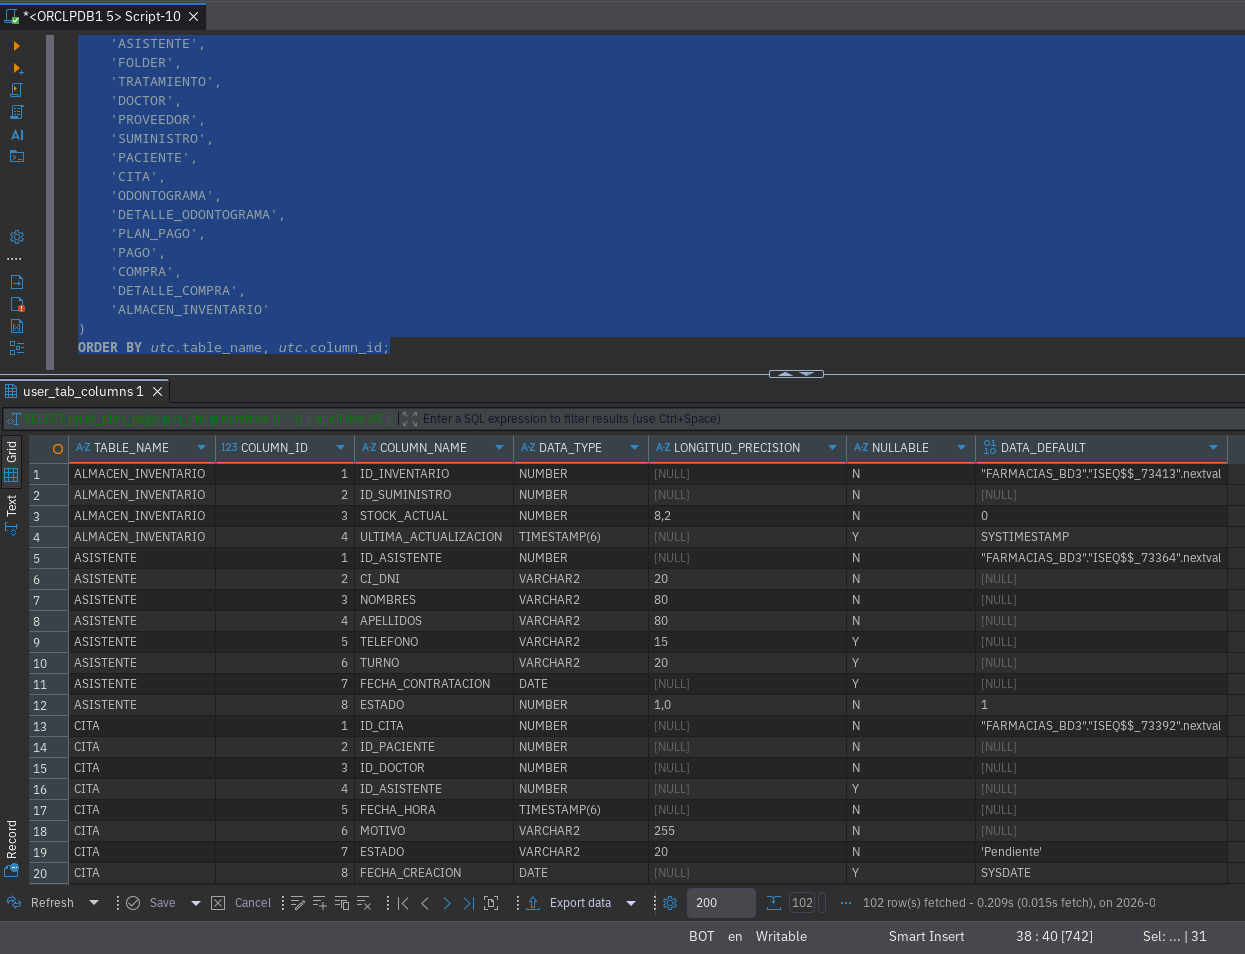
\includegraphics[width=\textwidth]{15_diccionario_tecnico_columnas.png}
\caption{Extracción técnica de columnas desde Oracle.}
\label{fig:diccionario-columnas}
\end{figure}

\begin{figure}[H]
\centering
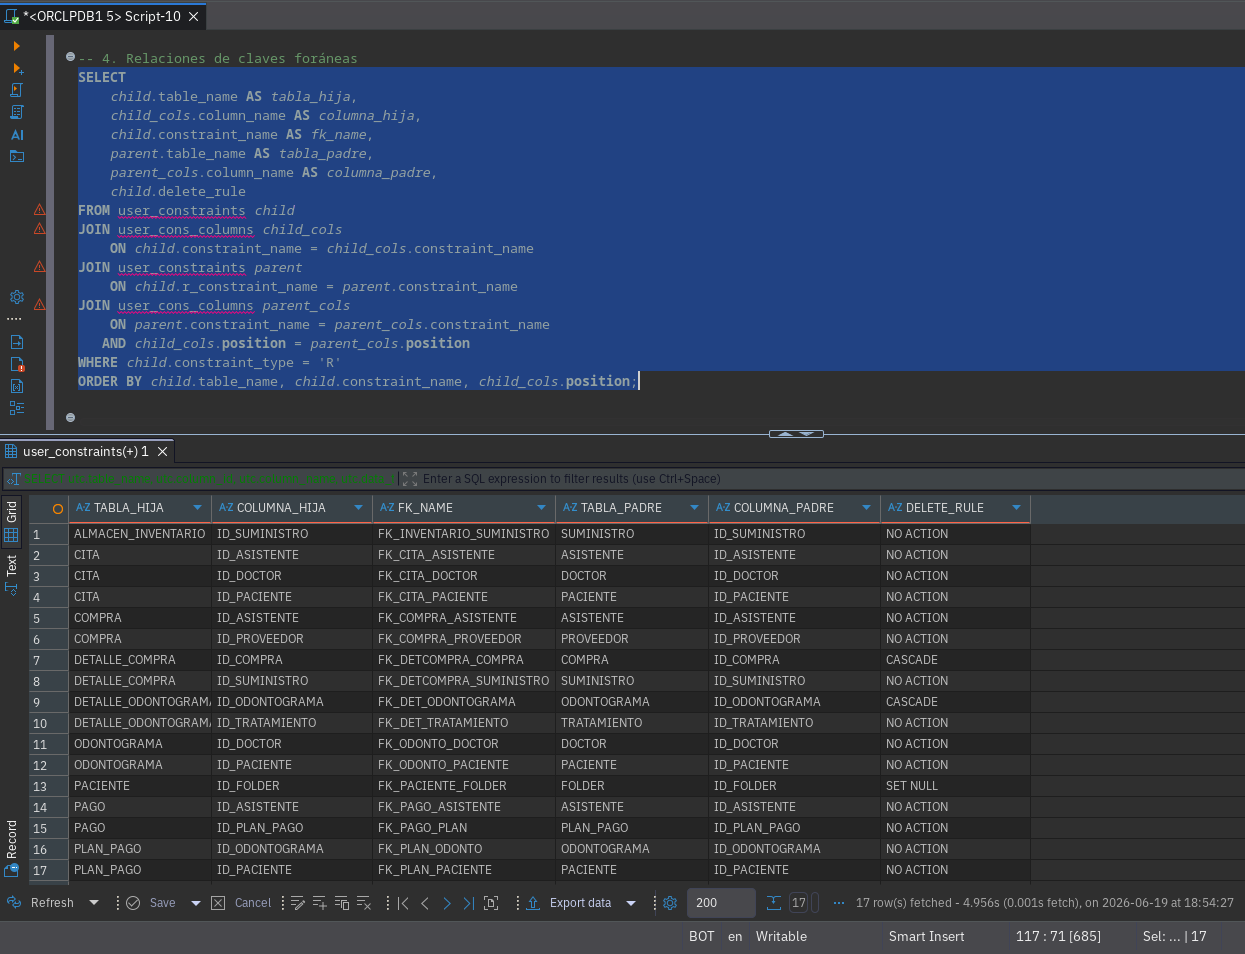
\includegraphics[width=\textwidth]{16_diccionario_tecnico_relaciones.png}
\caption{Extracción técnica de relaciones desde Oracle.}
\label{fig:diccionario-relaciones}
\end{figure}

\section{Validaciones}

Las validaciones se ejecutaron sobre Oracle Database 19c mediante DBeaver. Primero se validó la creación del schema, luego la creación de tablas, restricciones, vista, triggers y procedimiento. Posteriormente, se cargaron datos de prueba y se verificó el comportamiento del inventario y del registro de pagos.

\begin{figure}[H]
\centering
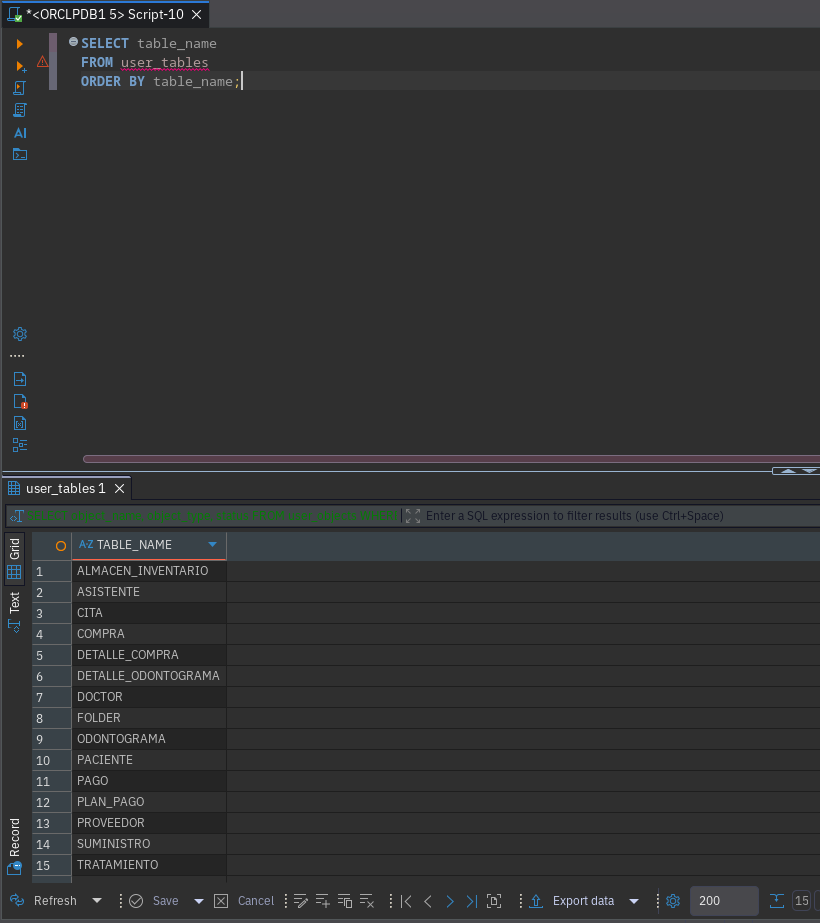
\includegraphics[width=\textwidth]{08_tablas_creadas_farmacias_bd3.png}
\caption{Tablas creadas en el schema FARMACIAS\_BD3.}
\label{fig:tablas-creadas}
\end{figure}

\begin{figure}[H]
\centering
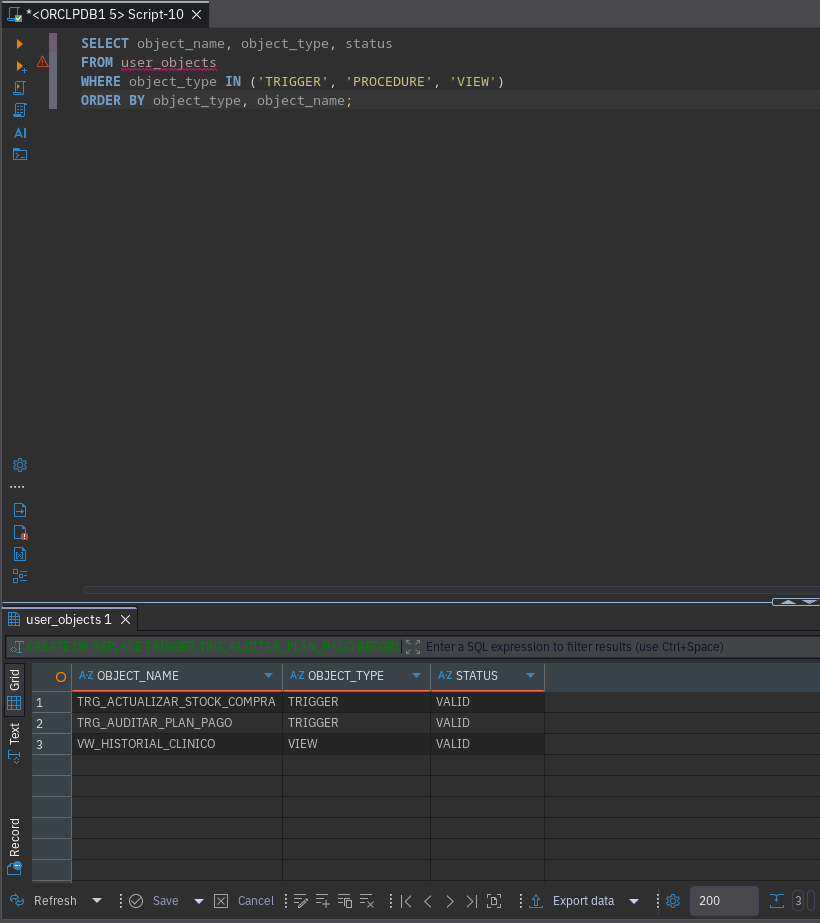
\includegraphics[width=\textwidth]{09_triggers_procedimiento_validos.png}
\caption{Vista y triggers validados en Oracle.}
\label{fig:triggers-validos}
\end{figure}

\begin{figure}[H]
\centering
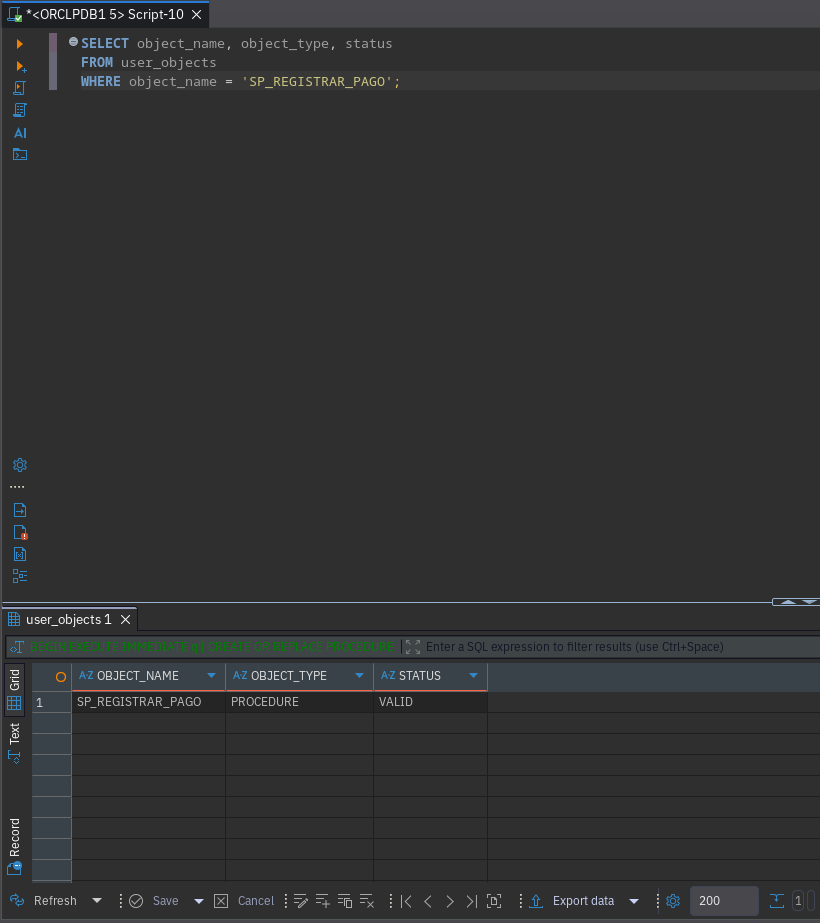
\includegraphics[width=\textwidth]{09a_procedimiento_registrar_pago_valido.png}
\caption{Procedimiento almacenado validado en Oracle.}
\label{fig:procedimiento-valido}
\end{figure}

\begin{figure}[H]
\centering
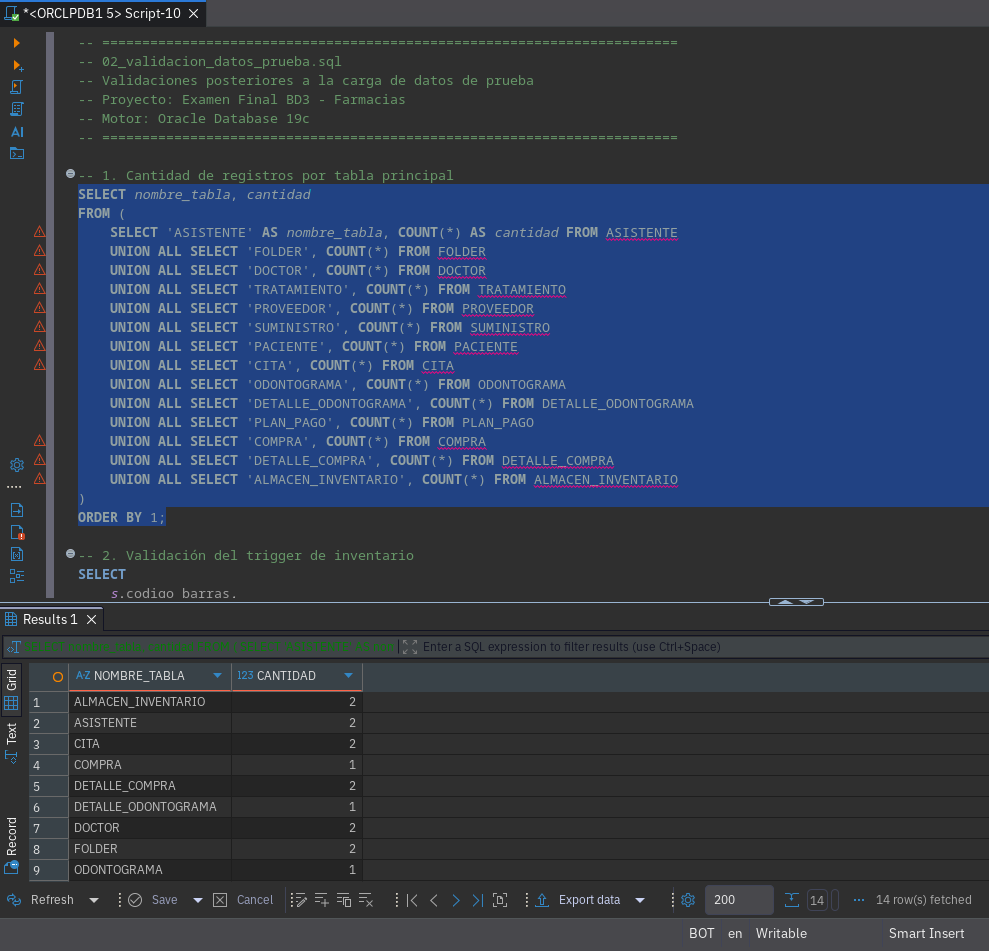
\includegraphics[width=\textwidth]{11_validacion_datos_prueba.png}
\caption{Validación de datos de prueba cargados.}
\label{fig:datos-prueba}
\end{figure}

\begin{figure}[H]
\centering
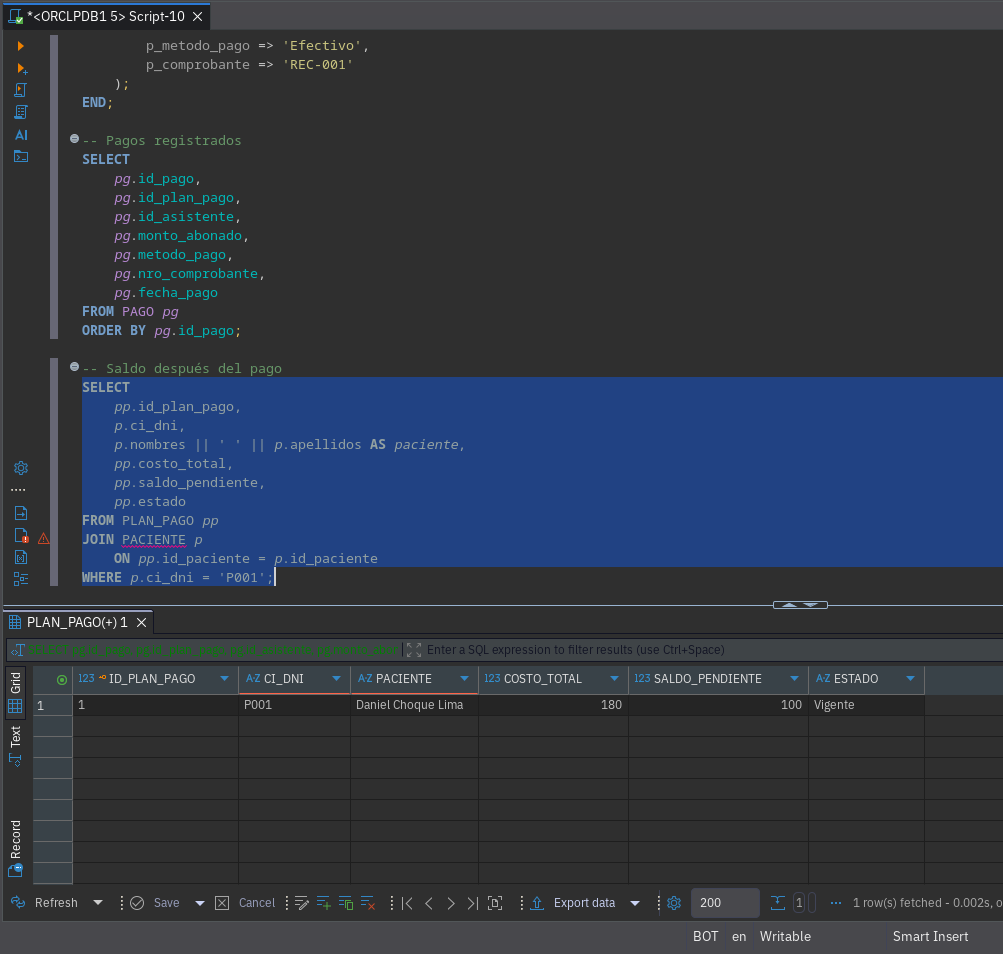
\includegraphics[width=\textwidth]{12_prueba_procedimiento_pago.png}
\caption{Prueba funcional del procedimiento de pago.}
\label{fig:prueba-pago}
\end{figure}

\section{Conversión del enfoque MySQL/Laravel de la tesis a Oracle 19c}

\subsection{Punto de partida documental}

La tesis base plantea un sistema web para el consultorio odontológico LALYSDENT. El sistema fue desarrollado con Laravel 11, Jetstream, Livewire, Tailwind CSS, JQuery y MySQL, bajo arquitectura MVC. Su alcance funcional incluye registro de pacientes, citas, historias clínicas, odontograma, tratamientos, inventario, pagos y reportes consolidados \parencite{tesisbase,calvocobos2025web}.

La conversión realizada en este proyecto toma ese dominio como referencia, pero cambia el foco: en lugar de documentar la aplicación web, se documenta la base de datos como producto principal. Por ello, el resultado no es una migración automática de un dump MySQL, sino una transformación técnica del diseño de datos hacia Oracle Database 19c.

\subsection{Diferencia de enfoque}

En el enfoque Laravel/MySQL, MySQL actúa como repositorio relacional para una aplicación web cuya lógica se distribuye entre modelos, controladores, vistas, componentes Livewire y validaciones del framework. En la transformación a Oracle 19c, varias reglas críticas se expresan directamente dentro del motor mediante restricciones, triggers, vista y procedimiento almacenado.

\begin{table}[H]
\caption{Cambio de enfoque entre MySQL/Laravel y Oracle 19c}
\centering
\small
\begin{tabularx}{\textwidth}{L{0.25\textwidth}Y Y}
\toprule
\textbf{Aspecto} & \textbf{MySQL/Laravel en la tesis} & \textbf{Oracle 19c en este proyecto} \\
\midrule
Propósito principal & Persistencia para un sistema web odontológico. & Diseño e implementación formal de base de datos. \\
Capa dominante & Aplicación Laravel bajo MVC. & Motor Oracle con SQL y PL/SQL. \\
Validaciones & Formularios, modelos, controladores y base de datos. & Restricciones, claves, triggers y procedimiento. \\
Automatización & Principalmente desde la lógica de aplicación. & Triggers y procedimiento almacenado. \\
Evidencia & Funcionalidad del sistema web. & Scripts, consultas, catálogo Oracle y datos de prueba. \\
\bottomrule
\end{tabularx}
\end{table}

\subsection{Conversión de tipos de datos}

La conversión física requirió adaptar tipos usados normalmente en MySQL o Laravel hacia tipos Oracle equivalentes. La tabla siguiente resume el criterio aplicado.

\begin{table}[H]
\caption{Conversión de tipos de datos hacia Oracle 19c}
\centering
\small
\begin{tabularx}{\textwidth}{L{0.28\textwidth}L{0.28\textwidth}Y}
\toprule
\textbf{Necesidad} & \textbf{MySQL/Laravel} & \textbf{Oracle 19c aplicado} \\
\midrule
Clave primaria autogenerada & \path{INT AUTO_INCREMENT} o migraciones Laravel con \path{id()}. & \path{NUMBER GENERATED ALWAYS AS IDENTITY}. \\
Texto variable & \path{VARCHAR}. & \path{VARCHAR2(n)}. \\
Texto fijo corto & \path{CHAR}. & \path{CHAR(1)}. \\
Fecha simple & \path{DATE}. & \path{DATE}. \\
Fecha y hora & \path{DATETIME} o \path{TIMESTAMP}. & \path{TIMESTAMP}. \\
Monto monetario & \path{DECIMAL(p,s)}. & \path{NUMBER(p,s)}. \\
Estado lógico & Booleano, tinyint o entero. & \path{NUMBER(1)} o \path{VARCHAR2} con restricción. \\
Fecha actual & \path{NOW()} o \path{CURRENT_TIMESTAMP}. & \path{SYSDATE} o \path{SYSTIMESTAMP}. \\
\bottomrule
\end{tabularx}
\end{table}

\subsection{Conversión de módulos funcionales a tablas Oracle}

Los módulos funcionales descritos en la tesis se transformaron en tablas y relaciones explícitas. El módulo de pacientes se convirtió en la tabla \texttt{PACIENTE}; la gestión documental se representó mediante \texttt{FOLDER}; las citas mediante \texttt{CITA}; la atención clínica mediante \texttt{ODONTOGRAMA} y \texttt{DETALLE\_ODONTOGRAMA}; los tratamientos mediante \texttt{TRATAMIENTO}; los pagos mediante \texttt{PLAN\_PAGO} y \texttt{PAGO}; y el inventario mediante \texttt{SUMINISTRO}, \texttt{COMPRA}, \texttt{DETALLE\_COMPRA} y \texttt{ALMACEN\_INVENTARIO}.

\begin{table}[H]
\caption{Transformación de módulos de la tesis a objetos Oracle}
\centering
\small
\begin{tabularx}{\textwidth}{L{0.30\textwidth}Y Y}
\toprule
\textbf{Módulo documentado} & \textbf{Interpretación de datos} & \textbf{Objeto Oracle resultante} \\
\midrule
Registro de pacientes & Datos personales, contacto y antecedentes. & \texttt{PACIENTE}. \\
Gestión de historias clínicas & Organización documental y clínica. & \texttt{FOLDER}, \texttt{ODONTOGRAMA}. \\
Citas odontológicas & Programación entre paciente, doctor y asistente. & \texttt{CITA}. \\
Odontograma & Evaluación dental por pieza, cara y diagnóstico. & \texttt{ODONTOGRAMA}, \texttt{DETALLE\_ODONTOGRAMA}. \\
Tratamientos & Catálogo clínico de tratamientos. & \texttt{TRATAMIENTO}. \\
Inventario odontológico & Suministros, compras y stock. & \texttt{SUMINISTRO}, \texttt{COMPRA}, \texttt{DETALLE\_COMPRA}, \texttt{ALMACEN\_INVENTARIO}. \\
Pagos de pacientes & Plan financiero y abonos realizados. & \texttt{PLAN\_PAGO}, \texttt{PAGO}. \\
Reportes consolidados & Consultas integradas de datos clínicos. & \texttt{VW\_HISTORIAL\_CLINICO}. \\
\bottomrule
\end{tabularx}
\end{table}

\subsection{Conversión de reglas de integridad}

En Laravel, muchas reglas pueden implementarse como validaciones de formulario, reglas de modelo o lógica de controlador. En Oracle 19c se decidió trasladar reglas críticas al motor para impedir inconsistencias aunque los datos sean manipulados desde DBeaver u otro cliente SQL.

\begin{table}[H]
\caption{Conversión de reglas de negocio a restricciones Oracle}
\centering
\small
\begin{tabularx}{\textwidth}{L{0.30\textwidth}Y Y}
\toprule
\textbf{Regla} & \textbf{Enfoque Laravel/MySQL} & \textbf{Implementación Oracle 19c} \\
\midrule
Documento único de paciente & Validación de formulario y restricción única. & \texttt{UNIQUE(PACIENTE.ci\_dni)}. \\
Doctor con correo único & Validación en aplicación o índice único. & \texttt{UNIQUE(DOCTOR.correo)}. \\
Estado válido de cita & Validación desde formulario o controlador. & \texttt{CHECK} sobre \texttt{CITA.estado}. \\
Pago positivo & Validación de entrada y regla de negocio. & \texttt{CHECK(monto\_abonado > 0)}. \\
Saldo no negativo & Lógica de aplicación. & Trigger \texttt{TRG\_AUDITAR\_PLAN\_PAGO}. \\
Compra actualiza inventario & Servicio o controlador Laravel. & Trigger \texttt{TRG\_ACTUALIZAR\_STOCK\_COMPRA}. \\
Registro de pago consistente & Transacción en aplicación. & Procedimiento \texttt{SP\_REGISTRAR\_PAGO}. \\
Consulta de historial clínico & Consulta desde modelos/controladores. & Vista \texttt{VW\_HISTORIAL\_CLINICO}. \\
\bottomrule
\end{tabularx}
\end{table}

\subsection{Conversión de relaciones}

Las relaciones que en Laravel podrían expresarse mediante modelos Eloquent se materializaron como claves foráneas en Oracle. La decisión permite que la integridad referencial no dependa únicamente de la aplicación.

\begin{itemize}
  \item \texttt{CITA} referencia a \texttt{PACIENTE}, \texttt{DOCTOR} y opcionalmente a \texttt{ASISTENTE}.
  \item \texttt{ODONTOGRAMA} referencia a \texttt{PACIENTE} y \texttt{DOCTOR}.
  \item \texttt{DETALLE\_ODONTOGRAMA} referencia a \texttt{ODONTOGRAMA} y opcionalmente a \texttt{TRATAMIENTO}.
  \item \texttt{PLAN\_PAGO} referencia a \texttt{PACIENTE} y \texttt{ODONTOGRAMA}.
  \item \texttt{PAGO} referencia a \texttt{PLAN\_PAGO} y opcionalmente a \texttt{ASISTENTE}.
  \item \texttt{COMPRA} referencia a \texttt{PROVEEDOR} y opcionalmente a \texttt{ASISTENTE}.
  \item \texttt{DETALLE\_COMPRA} referencia a \texttt{COMPRA} y \texttt{SUMINISTRO}.
  \item \texttt{ALMACEN\_INVENTARIO} referencia de forma única a \texttt{SUMINISTRO}.
\end{itemize}

\subsection{Resultado de la transformación}

El resultado final de la conversión es un schema Oracle llamado \texttt{FARMACIAS\_BD3}, compuesto por quince tablas, una vista, dos triggers, un procedimiento almacenado, scripts de datos de prueba y scripts de validación. Esta implementación permite demostrar no solo la estructura de datos, sino también el comportamiento del modelo ante operaciones reales como compras y pagos.

\subsection{Limitación de la comparación}

La comparación se basa en la tesis y en su sitio web de repositorio, no en un dump MySQL original. Por esa razón, las equivalencias se expresan a nivel de dominio, modelo de datos, tipos, reglas y objetos Oracle. No se presenta como una migración automática línea por línea.

\section{Ejecución del sistema Laravel de referencia}

Además de la tesis base y del repositorio académico de Calvo y Cobos, se clonó y ejecutó el repositorio Laravel propio del sistema odontológico LALYSDENT. Esta ejecución se realizó como verificación funcional de la aplicación web desarrollada por el equipo, no como reemplazo del diseño de base de datos desarrollado en este examen.

Se consideraron dos direcciones externas. La primera corresponde al repositorio académico de la tesis base, disponible en \url{https://calvocobos.github.io/}. La segunda corresponde al repositorio Laravel del proyecto, clonado y ejecutado localmente, disponible en \url{https://github.com/AlanDevPro/sistema-odontologico} \parencite{calvocobos2025web,sistemaodontologicogithub}.

\subsection{Relación con la tesis base}

La tesis base documenta un sistema de información web para la administración de procesos de registro, atención, inventario y finanzas del consultorio odontológico LALYSDENT. El repositorio Laravel del equipo permite complementar esa documentación con una aplicación funcional relacionada con el mismo dominio.

Sin embargo, el alcance del presente examen no consiste en reemplazar el objetivo del examen por la aplicación Laravel ni en adaptar su código al schema construido en este trabajo. El Laravel se ejecutó para verificar la aplicación web del proyecto y para fortalecer la comparación técnica entre el enfoque de aplicación web y el diseño de base de datos realizado en Oracle 19c.

\subsection{Separación entre schemas Oracle}

Para evitar mezclar responsabilidades, se usaron dos schemas distintos en Oracle:

\begin{table}[H]
\caption{Separación de schemas Oracle}
\centering
\small
\begin{tabularx}{\textwidth}{L{0.28\textwidth}Y}
\toprule
\textbf{Schema} & \textbf{Uso} \\
\midrule
\texttt{FARMACIAS\_BD3} & Schema diseñado, documentado y validado como producto principal del examen final. Contiene la base construida manualmente mediante SQL y PL/SQL. \\
\texttt{LALYSDENT\_APP} & Schema usado únicamente para ejecutar las migraciones y seeders del Laravel clonado. Permite comprobar la aplicación sin alterar el diseño del examen. \\
\bottomrule
\end{tabularx}
\end{table}

Esta separación es importante porque la aplicación Laravel ya posee su propia estructura de base de datos, sus migraciones y su lógica de aplicación. Por ello, no fue necesario conectarlo al schema \texttt{FARMACIAS\_BD3}.

\subsection{Entorno técnico verificado}

El repositorio Laravel fue ejecutado con PHP 8.5.7, Composer 2.9.2, Node.js 24.12.0, npm 11.6.2, Laravel Framework 12.62.0, Oracle Instant Client 19.31 y la extensión PHP OCI8 3.4.1. También se verificó la presencia de dependencias relevantes como \texttt{laravel/framework}, \texttt{laravel/jetstream}, \texttt{livewire/livewire} y \texttt{yajra/laravel-oci8}.

\figuranormal{20_laravel_entorno_php_node.png}
{Entorno PHP, Composer, Node.js, npm y módulos PHP para ejecutar Laravel.}
{fig:laravel-entorno}

\figuranormal{21_laravel_instantclient_oci8.png}
{Oracle Instant Client y extensión OCI8 habilitados en PHP.}
{fig:laravel-oci8}

\figuranormal{22_laravel_dependencias_ok.png}
{Dependencias Composer/npm y build del Laravel completados.}
{fig:laravel-dependencias}

\subsection{Conexión Oracle del Laravel}

El Laravel se configuró con conexión \texttt{oracle}, servicio \texttt{ORCLPDB1} y usuario \texttt{LALYSDENT\_APP}. Primero se validó la conexión directa desde PHP mediante OCI8; luego se verificó que Laravel leyera correctamente la conexión configurada en \texttt{.env} y \texttt{config/database.php}.

\figuranormal{25_laravel_conexion_oci8_lalysdent_app.png}
{Conexión OCI8 directa desde PHP al schema LALYSDENT\_APP.}
{fig:laravel-conexion-oci8}

\figuranormal{26_laravel_env_oracle_configurado.png}
{Laravel configurado con conexión oracle y servicio ORCLPDB1.}
{fig:laravel-env-oracle}

\subsection{Migraciones, seeders y datos}

Las migraciones del Laravel se ejecutaron sobre el schema \texttt{LALYSDENT\_APP}. Posteriormente, los seeders cargaron usuarios, pacientes, doctores, citas, tratamientos, pagos, proveedores, compras, suministros e inventario. Esto permitió verificar que la aplicación cuenta con datos de prueba propios.

\figuranormal{27_laravel_migraciones_seeders_ok.png}
{Migraciones y seeders ejecutados en Oracle desde Laravel.}
{fig:laravel-migraciones}

\figuranormal{28_laravel_usuarios_rutas.png}
{Usuarios de prueba generados por seeders y revisión de credenciales.}
{fig:laravel-usuarios}

\subsection{Aplicación web funcionando}

Después de levantar el servidor local con \path{php artisan serve}, se verificó la pantalla pública, el inicio de sesión, el panel principal y el módulo de pacientes. Estas evidencias muestran que el Laravel funciona como sistema web independiente.

\figuranormal{29_laravel_pantalla_inicio_login.png}
{Pantalla pública e ingreso al sistema Laravel.}
{fig:laravel-login}

\figuranormal{30_laravel_dashboard_funcionando.png}
{Panel principal del sistema Laravel funcionando.}
{fig:laravel-dashboard}

\figuranormal{31_laravel_modulo_datos_seeders.png}
{Módulo de pacientes con datos cargados desde seeders.}
{fig:laravel-pacientes}

\subsection{Resultado}

La ejecución del Laravel confirma que la aplicación Laravel del proyecto funciona correctamente en el dominio odontológico. Sin embargo, el objetivo principal de este informe sigue siendo el diseño, transformación, implementación y validación de la base de datos Oracle 19c desarrollada para el examen. El Laravel se documenta como implementación web propia, evidencia funcional complementaria y punto de comparación frente al diseño independiente realizado en \texttt{FARMACIAS\_BD3}.

\section{Fuentes del trabajo}

En este informe, el término fuentes se refiere a los archivos, diagramas, scripts y evidencias generados durante el desarrollo del proyecto. Estos artefactos se encuentran organizados dentro del repositorio del examen final.

\begin{table}[H]
\caption{Fuentes y artefactos del trabajo}
\centering
\small
\begin{tabularx}{\textwidth}{L{0.30\textwidth}Y}
\toprule
\textbf{Categoría} & \textbf{Archivo o evidencia} \\
\midrule
Requisitos & \path{00_requisitos/01_alcance_y_supuestos.md} \\
Modelo Chen editable & \path{01_conceptual_chen/modelo_conceptual_chen_bd3.drawio} \\
Modelo Chen exportado & \path{01_conceptual_chen/modelo_chen_*.png} \\
Transformación lógica & \path{02_transformacion_logica/01_transformacion_modelo_relacional.md} \\
Modelo Crow's Foot & \path{03_crows_foot/modelo_logico_crows_foot_bd3.DM1} \\
Modelo Crow's Foot exportado & \path{03_crows_foot/modelo_logico_crows_foot_bd3.jpg} \\
DDL y PL/SQL Oracle & \path{05_oracle_ddl/*.sql} \\
Evidencias & \path{06_evidencias/*.png} \\
Diccionario de datos & \path{08_diccionario_datos/01_diccionario_datos.md} \\
Comparación MySQL/Oracle & \path{09_comparacion_mysql_oracle/*.md} \\
Validaciones & \path{10_validaciones/*.sql} \\
\bottomrule
\end{tabularx}
\end{table}

\section{Conclusiones}

Se diseñó e implementó una base de datos relacional para procesos odontológicos, cubriendo registro de pacientes, citas, odontogramas, tratamientos, pagos, compras e inventario.

El modelo conceptual Chen permitió representar el dominio sin depender de un motor físico. La transformación relacional permitió derivar tablas, claves y relaciones. El modelo lógico Crow's Foot facilitó la visualización de la estructura relacional, mientras que Oracle Database 19c permitió implementar el diseño físico con restricciones, vista, triggers y procedimiento almacenado.

Las validaciones realizadas demostraron que los objetos fueron creados correctamente y que las reglas implementadas funcionan. En particular, se verificó la actualización de inventario al registrar compras y la actualización de saldo al registrar pagos mediante el procedimiento \texttt{SP\_REGISTRAR\_PAGO}.

Finalmente, la comparación con el enfoque MySQL/Laravel descrito en la tesis base permitió evidenciar que Oracle 19c ofrece una implementación más centrada en reglas del motor, integridad relacional explícita y validación técnica mediante el catálogo de base de datos.


La ejecución del repositorio Laravel del proyecto permitió comprobar una aplicación funcional del mismo dominio odontológico usando Oracle, migraciones, seeders y autenticación. Esta verificación no sustituye la base diseñada en el examen; más bien, refuerza la trazabilidad entre el sistema web del proyecto LALYSDENT y el diseño independiente implementado en el schema \texttt{FARMACIAS\_BD3}.

El uso de schemas separados permitió mantener una distinción clara entre \texttt{FARMACIAS\_BD3}, como producto principal del examen, y \texttt{LALYSDENT\_APP}, como entorno de ejecución de la aplicación Laravel desarrollada por el equipo.


\clearpage
\printbibliography

\appendix
\section{Anexo: scripts SQL}

\subsection{Creación de schema/usuario}

\lstinputlisting[language=SQL]{../05_oracle_ddl/00_admin_crear_schema.sql}

\subsection{DDL físico Oracle 19c}

\lstinputlisting[language=SQL]{../05_oracle_ddl/02_tablas.sql}

\subsection{Vista}

\lstinputlisting[language=SQL]{../05_oracle_ddl/03_vistas.sql}

\subsection{Triggers}

\lstinputlisting[language=SQL]{../05_oracle_ddl/04_triggers.sql}

\subsection{Procedimiento almacenado}

\lstinputlisting[language=SQL]{../05_oracle_ddl/05_procedimientos.sql}

\subsection{Datos de prueba}

\lstinputlisting[language=SQL]{../05_oracle_ddl/06_datos_prueba.sql}

\section{Anexo: diccionario de datos completo}

El diccionario de datos completo se incluye como anexo para mantener trazabilidad entre la documentación técnica y el esquema implementado. A diferencia del archivo fuente en formato Markdown, en este anexo las tablas fueron convertidas a formato LaTeX para que se visualicen correctamente dentro del PDF final.

\begingroup
\scriptsize
\setlength{\tabcolsep}{2.5pt}
\renewcommand{\arraystretch}{1.15}
\subsection{Diccionario de datos}

\subsubsection{Descripción general}

El presente diccionario de datos documenta las tablas, columnas, tipos de datos, claves, restricciones y propósito funcional del esquema implementado en Oracle Database 19c. El modelo físico corresponde a una base de datos orientada a la administración de procesos de registro, atención clínica odontológica, inventario y pagos.\par

Aunque el schema del proyecto se denomina \texttt{FARMACIAS\_BD3} por convención del repositorio y del entorno académico, las entidades implementadas corresponden al dominio del sistema odontológico analizado a partir de la tesis base.\par



\subsubsection{Tabla: ASISTENTE}

\textbf{Propósito:} almacena los datos del personal asistente que participa en la gestión de citas, compras y pagos.\par

\begin{longtable}{p{0.18\linewidth}p{0.18\linewidth}p{0.08\linewidth}p{0.08\linewidth}p{0.36\linewidth}}
\toprule
\textbf{Campo} & \textbf{Tipo Oracle} & \textbf{Nulo} & \textbf{Clave} & \textbf{Descripción} \\
\midrule
\endfirsthead
\toprule
\textbf{Campo} & \textbf{Tipo Oracle} & \textbf{Nulo} & \textbf{Clave} & \textbf{Descripción} \\
\midrule
\endhead
id\_asistente & NUMBER & No & PK & Identificador único generado automáticamente. \\
ci\_dni & VARCHAR2(20) & No & UK & Documento de identidad del asistente. \\
nombres & VARCHAR2(80) & No &  & Nombres del asistente. \\
apellidos & VARCHAR2(80) & No &  & Apellidos del asistente. \\
telefono & VARCHAR2(15) & Sí &  & Número telefónico de contacto. \\
turno & VARCHAR2(20) & Sí &  & Turno asignado al asistente. \\
fecha\_contratacion & DATE & Sí &  & Fecha de contratación. \\
estado & NUMBER(1) & No &  & Estado lógico del registro. Valor por defecto: 1. \\
\bottomrule
\end{longtable}



\subsubsection{Tabla: FOLDER}

\textbf{Propósito:} representa el archivador o carpeta física/digital donde se ubica la documentación clínica del paciente.\par

\begin{longtable}{p{0.18\linewidth}p{0.18\linewidth}p{0.08\linewidth}p{0.08\linewidth}p{0.36\linewidth}}
\toprule
\textbf{Campo} & \textbf{Tipo Oracle} & \textbf{Nulo} & \textbf{Clave} & \textbf{Descripción} \\
\midrule
\endfirsthead
\toprule
\textbf{Campo} & \textbf{Tipo Oracle} & \textbf{Nulo} & \textbf{Clave} & \textbf{Descripción} \\
\midrule
\endhead
id\_folder & NUMBER & No & PK & Identificador único generado automáticamente. \\
codigo\_archivo & VARCHAR2(20) & No & UK & Código único del archivador o carpeta. \\
estante & VARCHAR2(20) & Sí &  & Estante donde se ubica el archivo. \\
seccion & VARCHAR2(20) & Sí &  & Sección dentro del estante. \\
observaciones & VARCHAR2(255) & Sí &  & Notas adicionales sobre el archivo. \\
\bottomrule
\end{longtable}



\subsubsection{Tabla: TRATAMIENTO}

\textbf{Propósito:} catálogo de tratamientos odontológicos disponibles.\par

\begin{longtable}{p{0.18\linewidth}p{0.18\linewidth}p{0.08\linewidth}p{0.08\linewidth}p{0.36\linewidth}}
\toprule
\textbf{Campo} & \textbf{Tipo Oracle} & \textbf{Nulo} & \textbf{Clave} & \textbf{Descripción} \\
\midrule
\endfirsthead
\toprule
\textbf{Campo} & \textbf{Tipo Oracle} & \textbf{Nulo} & \textbf{Clave} & \textbf{Descripción} \\
\midrule
\endhead
id\_tratamiento & NUMBER & No & PK & Identificador único generado automáticamente. \\
nombre & VARCHAR2(100) & No &  & Nombre del tratamiento. \\
descripcion & VARCHAR2(255) & Sí &  & Descripción breve del tratamiento. \\
costo\_referencial & NUMBER(10,2) & No &  & Costo referencial del tratamiento. \\
estado & NUMBER(1) & No &  & Estado lógico del tratamiento. Valor por defecto: 1. \\
\bottomrule
\end{longtable}



\subsubsection{Tabla: DOCTOR}

\textbf{Propósito:} almacena los datos de los doctores u odontólogos que atienden pacientes y registran odontogramas.\par

\begin{longtable}{p{0.18\linewidth}p{0.18\linewidth}p{0.08\linewidth}p{0.08\linewidth}p{0.36\linewidth}}
\toprule
\textbf{Campo} & \textbf{Tipo Oracle} & \textbf{Nulo} & \textbf{Clave} & \textbf{Descripción} \\
\midrule
\endfirsthead
\toprule
\textbf{Campo} & \textbf{Tipo Oracle} & \textbf{Nulo} & \textbf{Clave} & \textbf{Descripción} \\
\midrule
\endhead
id\_doctor & NUMBER & No & PK & Identificador único generado automáticamente. \\
ci\_dni & VARCHAR2(20) & No & UK & Documento de identidad del doctor. \\
nombres & VARCHAR2(80) & No &  & Nombres del doctor. \\
apellidos & VARCHAR2(80) & No &  & Apellidos del doctor. \\
especialidad & VARCHAR2(100) & Sí &  & Especialidad odontológica. \\
telefono & VARCHAR2(15) & Sí &  & Teléfono de contacto. \\
correo & VARCHAR2(100) & Sí & UK & Correo electrónico único. \\
estado & NUMBER(1) & No &  & Estado lógico del registro. Valor por defecto: 1. \\
\bottomrule
\end{longtable}



\subsubsection{Tabla: PROVEEDOR}

\textbf{Propósito:} almacena proveedores de suministros, materiales e insumos.\par

\begin{longtable}{p{0.18\linewidth}p{0.18\linewidth}p{0.08\linewidth}p{0.08\linewidth}p{0.36\linewidth}}
\toprule
\textbf{Campo} & \textbf{Tipo Oracle} & \textbf{Nulo} & \textbf{Clave} & \textbf{Descripción} \\
\midrule
\endfirsthead
\toprule
\textbf{Campo} & \textbf{Tipo Oracle} & \textbf{Nulo} & \textbf{Clave} & \textbf{Descripción} \\
\midrule
\endhead
id\_proveedor & NUMBER & No & PK & Identificador único generado automáticamente. \\
nit\_ruc & VARCHAR2(20) & No & UK & Número de identificación tributaria del proveedor. \\
razon\_social & VARCHAR2(100) & No &  & Razón social del proveedor. \\
nombre\_contacto & VARCHAR2(80) & Sí &  & Nombre de la persona de contacto. \\
telefono & VARCHAR2(15) & Sí &  & Teléfono de contacto. \\
direccion & VARCHAR2(255) & Sí &  & Dirección del proveedor. \\
correo & VARCHAR2(100) & Sí &  & Correo electrónico del proveedor. \\
\bottomrule
\end{longtable}



\subsubsection{Tabla: SUMINISTRO}

\textbf{Propósito:} catálogo de suministros utilizados en la atención odontológica y administración del inventario.\par

\begin{longtable}{p{0.18\linewidth}p{0.18\linewidth}p{0.08\linewidth}p{0.08\linewidth}p{0.36\linewidth}}
\toprule
\textbf{Campo} & \textbf{Tipo Oracle} & \textbf{Nulo} & \textbf{Clave} & \textbf{Descripción} \\
\midrule
\endfirsthead
\toprule
\textbf{Campo} & \textbf{Tipo Oracle} & \textbf{Nulo} & \textbf{Clave} & \textbf{Descripción} \\
\midrule
\endhead
id\_suministro & NUMBER & No & PK & Identificador único generado automáticamente. \\
codigo\_barras & VARCHAR2(50) & Sí & UK & Código de barras o código interno del suministro. \\
nombre & VARCHAR2(100) & No &  & Nombre del suministro. \\
categoria & VARCHAR2(50) & Sí &  & Categoría del suministro. \\
unidad\_medida & VARCHAR2(20) & Sí &  & Unidad de medida usada para controlar stock. \\
stock\_minimo & NUMBER(5) & No &  & Cantidad mínima recomendada en inventario. \\
estado & NUMBER(1) & No &  & Estado lógico del suministro. Valor por defecto: 1. \\
\bottomrule
\end{longtable}



\subsubsection{Tabla: PACIENTE}

\textbf{Propósito:} registra los datos personales y antecedentes clínicos básicos de los pacientes.\par

\begin{longtable}{p{0.18\linewidth}p{0.18\linewidth}p{0.08\linewidth}p{0.08\linewidth}p{0.36\linewidth}}
\toprule
\textbf{Campo} & \textbf{Tipo Oracle} & \textbf{Nulo} & \textbf{Clave} & \textbf{Descripción} \\
\midrule
\endfirsthead
\toprule
\textbf{Campo} & \textbf{Tipo Oracle} & \textbf{Nulo} & \textbf{Clave} & \textbf{Descripción} \\
\midrule
\endhead
id\_paciente & NUMBER & No & PK & Identificador único generado automáticamente. \\
id\_folder & NUMBER & Sí & FK & Referencia al archivador físico o digital del paciente. \\
ci\_dni & VARCHAR2(20) & No & UK & Documento de identidad del paciente. \\
nombres & VARCHAR2(80) & No &  & Nombres del paciente. \\
apellidos & VARCHAR2(80) & No &  & Apellidos del paciente. \\
fecha\_nacimiento & DATE & No &  & Fecha de nacimiento. \\
sexo & CHAR(1) & Sí &  & Sexo registrado del paciente. \\
telefono & VARCHAR2(15) & Sí &  & Teléfono de contacto. \\
direccion & VARCHAR2(255) & Sí &  & Dirección del paciente. \\
antecedentes\_medicos & VARCHAR2(500) & Sí &  & Antecedentes médicos declarados. \\
fecha\_registro & DATE & Sí &  & Fecha de registro del paciente. Valor por defecto: SYSDATE. \\
\bottomrule
\end{longtable}

\textbf{Relaciones:}\par
\texttt{PACIENTE.id\_folder} referencia \texttt{FOLDER.id\_folder} con \texttt{ON DELETE SET NULL}.\par



\subsubsection{Tabla: CITA}

\textbf{Propósito:} registra la programación de atenciones odontológicas.\par

\begin{longtable}{p{0.18\linewidth}p{0.18\linewidth}p{0.08\linewidth}p{0.08\linewidth}p{0.36\linewidth}}
\toprule
\textbf{Campo} & \textbf{Tipo Oracle} & \textbf{Nulo} & \textbf{Clave} & \textbf{Descripción} \\
\midrule
\endfirsthead
\toprule
\textbf{Campo} & \textbf{Tipo Oracle} & \textbf{Nulo} & \textbf{Clave} & \textbf{Descripción} \\
\midrule
\endhead
id\_cita & NUMBER & No & PK & Identificador único generado automáticamente. \\
id\_paciente & NUMBER & No & FK & Paciente citado. \\
id\_doctor & NUMBER & No & FK & Doctor asignado. \\
id\_asistente & NUMBER & Sí & FK & Asistente relacionado con la cita. \\
fecha\_hora & TIMESTAMP & No &  & Fecha y hora programada. \\
motivo & VARCHAR2(255) & No &  & Motivo de la cita. \\
estado & VARCHAR2(20) & No & CHECK & Estado de la cita. \\
fecha\_creacion & DATE & Sí &  & Fecha de creación del registro. Valor por defecto: SYSDATE. \\
\bottomrule
\end{longtable}

\textbf{Valores permitidos para estado:} \texttt{Pendiente}, \texttt{Confirmada}, \texttt{Atendida}, \texttt{Cancelada}, \texttt{Reprogramada}.\par

\textbf{Relaciones:}\par
\texttt{CITA.id\_paciente} referencia \texttt{PACIENTE.id\_paciente}.\par
\texttt{CITA.id\_doctor} referencia \texttt{DOCTOR.id\_doctor}.\par
\texttt{CITA.id\_asistente} referencia \texttt{ASISTENTE.id\_asistente}.\par



\subsubsection{Tabla: ODONTOGRAMA}

\textbf{Propósito:} representa la evaluación odontológica general de un paciente.\par

\begin{longtable}{p{0.18\linewidth}p{0.18\linewidth}p{0.08\linewidth}p{0.08\linewidth}p{0.36\linewidth}}
\toprule
\textbf{Campo} & \textbf{Tipo Oracle} & \textbf{Nulo} & \textbf{Clave} & \textbf{Descripción} \\
\midrule
\endfirsthead
\toprule
\textbf{Campo} & \textbf{Tipo Oracle} & \textbf{Nulo} & \textbf{Clave} & \textbf{Descripción} \\
\midrule
\endhead
id\_odontograma & NUMBER & No & PK & Identificador único generado automáticamente. \\
id\_paciente & NUMBER & No & FK & Paciente evaluado. \\
id\_doctor & NUMBER & No & FK & Doctor que registra la evaluación. \\
fecha\_evaluacion & DATE & No &  & Fecha de evaluación. Valor por defecto: SYSDATE. \\
observaciones\_generales & VARCHAR2(500) & Sí &  & Observaciones clínicas generales. \\
\bottomrule
\end{longtable}

\textbf{Relaciones:}\par
\texttt{ODONTOGRAMA.id\_paciente} referencia \texttt{PACIENTE.id\_paciente}.\par
\texttt{ODONTOGRAMA.id\_doctor} referencia \texttt{DOCTOR.id\_doctor}.\par



\subsubsection{Tabla: DETALLE\_ODONTOGRAMA}

\textbf{Propósito:} registra el detalle clínico por pieza dental, cara, diagnóstico y tratamiento asociado.\par

\begin{longtable}{p{0.18\linewidth}p{0.18\linewidth}p{0.08\linewidth}p{0.08\linewidth}p{0.36\linewidth}}
\toprule
\textbf{Campo} & \textbf{Tipo Oracle} & \textbf{Nulo} & \textbf{Clave} & \textbf{Descripción} \\
\midrule
\endfirsthead
\toprule
\textbf{Campo} & \textbf{Tipo Oracle} & \textbf{Nulo} & \textbf{Clave} & \textbf{Descripción} \\
\midrule
\endhead
id\_detalle & NUMBER & No & PK & Identificador único generado automáticamente. \\
id\_odontograma & NUMBER & No & FK & Odontograma al que pertenece el detalle. \\
id\_tratamiento & NUMBER & Sí & FK & Tratamiento asociado, si corresponde. \\
pieza\_dental & VARCHAR2(10) & No &  & Código o número de pieza dental. \\
cara & VARCHAR2(20) & No &  & Cara dental evaluada. \\
diagnostico & VARCHAR2(100) & No &  & Diagnóstico registrado. \\
estado & VARCHAR2(20) & Sí &  & Estado del tratamiento o atención. Valor por defecto: Por tratar. \\
\bottomrule
\end{longtable}

\textbf{Relaciones:}\par
\texttt{DETALLE\_ODONTOGRAMA.id\_odontograma} referencia \texttt{ODONTOGRAMA.id\_odontograma} con \texttt{ON DELETE CASCADE}.\par
\texttt{DETALLE\_ODONTOGRAMA.id\_tratamiento} referencia \texttt{TRATAMIENTO.id\_tratamiento}.\par



\subsubsection{Tabla: PLAN\_PAGO}

\textbf{Propósito:} registra el costo total y saldo pendiente de los tratamientos asociados a un odontograma.\par

\begin{longtable}{p{0.18\linewidth}p{0.18\linewidth}p{0.08\linewidth}p{0.08\linewidth}p{0.36\linewidth}}
\toprule
\textbf{Campo} & \textbf{Tipo Oracle} & \textbf{Nulo} & \textbf{Clave} & \textbf{Descripción} \\
\midrule
\endfirsthead
\toprule
\textbf{Campo} & \textbf{Tipo Oracle} & \textbf{Nulo} & \textbf{Clave} & \textbf{Descripción} \\
\midrule
\endhead
id\_plan\_pago & NUMBER & No & PK & Identificador único generado automáticamente. \\
id\_paciente & NUMBER & No & FK & Paciente asociado al plan. \\
id\_odontograma & NUMBER & No & FK & Odontograma relacionado. \\
fecha\_creacion & DATE & Sí &  & Fecha de creación del plan. Valor por defecto: SYSDATE. \\
costo\_total & NUMBER(10,2) & No &  & Costo total del plan. \\
saldo\_pendiente & NUMBER(10,2) & No &  & Saldo pendiente de pago. \\
estado & VARCHAR2(20) & Sí &  & Estado del plan. Valor por defecto: Vigente. \\
\bottomrule
\end{longtable}

\textbf{Relaciones:}\par
\texttt{PLAN\_PAGO.id\_paciente} referencia \texttt{PACIENTE.id\_paciente}.\par
\texttt{PLAN\_PAGO.id\_odontograma} referencia \texttt{ODONTOGRAMA.id\_odontograma}.\par

\textbf{Regla automatizada:}\par
El trigger \texttt{TRG\_AUDITAR\_PLAN\_PAGO} impide que el saldo pendiente sea negativo y cambia el estado a \texttt{Pagado} cuando el saldo llega a cero.\par



\subsubsection{Tabla: PAGO}

\textbf{Propósito:} registra los pagos efectuados por los pacientes sobre un plan de pago.\par

\begin{longtable}{p{0.18\linewidth}p{0.18\linewidth}p{0.08\linewidth}p{0.08\linewidth}p{0.36\linewidth}}
\toprule
\textbf{Campo} & \textbf{Tipo Oracle} & \textbf{Nulo} & \textbf{Clave} & \textbf{Descripción} \\
\midrule
\endfirsthead
\toprule
\textbf{Campo} & \textbf{Tipo Oracle} & \textbf{Nulo} & \textbf{Clave} & \textbf{Descripción} \\
\midrule
\endhead
id\_pago & NUMBER & No & PK & Identificador único generado automáticamente. \\
id\_plan\_pago & NUMBER & No & FK & Plan de pago asociado. \\
id\_asistente & NUMBER & Sí & FK & Asistente que registra el pago. \\
fecha\_pago & TIMESTAMP & No &  & Fecha y hora del pago. Valor por defecto: SYSTIMESTAMP. \\
monto\_abonado & NUMBER(10,2) & No & CHECK & Monto abonado. Debe ser mayor a cero. \\
metodo\_pago & VARCHAR2(30) & No &  & Método de pago utilizado. \\
nro\_comprobante & VARCHAR2(50) & Sí &  & Número de recibo o comprobante. \\
\bottomrule
\end{longtable}

\textbf{Relaciones:}\par
\texttt{PAGO.id\_plan\_pago} referencia \texttt{PLAN\_PAGO.id\_plan\_pago}.\par
\texttt{PAGO.id\_asistente} referencia \texttt{ASISTENTE.id\_asistente}.\par

\textbf{Regla:}\par
\texttt{CHK\_MONTO\_PAGO} exige que \texttt{monto\_abonado \textgreater{} 0}.\par



\subsubsection{Tabla: COMPRA}

\textbf{Propósito:} registra compras de suministros realizadas a proveedores.\par

\begin{longtable}{p{0.18\linewidth}p{0.18\linewidth}p{0.08\linewidth}p{0.08\linewidth}p{0.36\linewidth}}
\toprule
\textbf{Campo} & \textbf{Tipo Oracle} & \textbf{Nulo} & \textbf{Clave} & \textbf{Descripción} \\
\midrule
\endfirsthead
\toprule
\textbf{Campo} & \textbf{Tipo Oracle} & \textbf{Nulo} & \textbf{Clave} & \textbf{Descripción} \\
\midrule
\endhead
id\_compra & NUMBER & No & PK & Identificador único generado automáticamente. \\
id\_proveedor & NUMBER & No & FK & Proveedor de la compra. \\
id\_asistente & NUMBER & Sí & FK & Asistente que registra la compra. \\
fecha\_compra & DATE & No &  & Fecha de la compra. \\
nro\_factura & VARCHAR2(50) & Sí &  & Número de factura. \\
total\_compra & NUMBER(10,2) & No &  & Total monetario de la compra. \\
estado & VARCHAR2(20) & Sí &  & Estado de la compra. Valor por defecto: Completada. \\
\bottomrule
\end{longtable}

\textbf{Relaciones:}\par
\texttt{COMPRA.id\_proveedor} referencia \texttt{PROVEEDOR.id\_proveedor}.\par
\texttt{COMPRA.id\_asistente} referencia \texttt{ASISTENTE.id\_asistente}.\par



\subsubsection{Tabla: DETALLE\_COMPRA}

\textbf{Propósito:} registra los suministros incluidos en cada compra.\par

\begin{longtable}{p{0.18\linewidth}p{0.18\linewidth}p{0.08\linewidth}p{0.08\linewidth}p{0.36\linewidth}}
\toprule
\textbf{Campo} & \textbf{Tipo Oracle} & \textbf{Nulo} & \textbf{Clave} & \textbf{Descripción} \\
\midrule
\endfirsthead
\toprule
\textbf{Campo} & \textbf{Tipo Oracle} & \textbf{Nulo} & \textbf{Clave} & \textbf{Descripción} \\
\midrule
\endhead
id\_detalle\_compra & NUMBER & No & PK & Identificador único generado automáticamente. \\
id\_compra & NUMBER & No & FK & Compra a la que pertenece el detalle. \\
id\_suministro & NUMBER & No & FK & Suministro comprado. \\
cantidad & NUMBER(8,2) & No &  & Cantidad comprada. \\
precio\_unitario & NUMBER(10,2) & No &  & Precio unitario del suministro. \\
subtotal & NUMBER(10,2) & No &  & Subtotal del detalle. \\
\bottomrule
\end{longtable}

\textbf{Relaciones:}\par
\texttt{DETALLE\_COMPRA.id\_compra} referencia \texttt{COMPRA.id\_compra} con \texttt{ON DELETE CASCADE}.\par
\texttt{DETALLE\_COMPRA.id\_suministro} referencia \texttt{SUMINISTRO.id\_suministro}.\par

\textbf{Regla automatizada:}\par
El trigger \texttt{TRG\_ACTUALIZAR\_STOCK\_COMPRA} actualiza o crea el registro correspondiente en \texttt{ALMACEN\_INVENTARIO} después de insertar un detalle de compra.\par



\subsubsection{Tabla: ALMACEN\_INVENTARIO}

\textbf{Propósito:} controla el stock actual por suministro.\par

\begin{longtable}{p{0.18\linewidth}p{0.18\linewidth}p{0.08\linewidth}p{0.08\linewidth}p{0.36\linewidth}}
\toprule
\textbf{Campo} & \textbf{Tipo Oracle} & \textbf{Nulo} & \textbf{Clave} & \textbf{Descripción} \\
\midrule
\endfirsthead
\toprule
\textbf{Campo} & \textbf{Tipo Oracle} & \textbf{Nulo} & \textbf{Clave} & \textbf{Descripción} \\
\midrule
\endhead
id\_inventario & NUMBER & No & PK & Identificador único generado automáticamente. \\
id\_suministro & NUMBER & No & FK / UK & Suministro inventariado. Debe ser único en inventario. \\
stock\_actual & NUMBER(8,2) & No &  & Stock disponible actual. \\
ultima\_actualizacion & TIMESTAMP & Sí &  & Fecha y hora de última actualización. Valor por defecto: SYSTIMESTAMP. \\
\bottomrule
\end{longtable}

\textbf{Relaciones:}\par
\texttt{ALMACEN\_INVENTARIO.id\_suministro} referencia \texttt{SUMINISTRO.id\_suministro}.\par



\subsubsection{Vista: VW\_HISTORIAL\_CLINICO}

\textbf{Propósito:} integra información de pacientes, doctores, odontogramas, detalles clínicos y tratamientos para consultar el historial clínico odontológico.\par

\begin{longtable}{p{0.46\linewidth}p{0.46\linewidth}}
\toprule
\textbf{Columna} & \textbf{Descripción} \\
\midrule
\endfirsthead
\toprule
\textbf{Columna} & \textbf{Descripción} \\
\midrule
\endhead
dni\_paciente & Documento de identidad del paciente. \\
nombre\_paciente & Nombre completo del paciente. \\
doctor\_tratante & Nombre completo del doctor tratante. \\
fecha\_evaluacion & Fecha de evaluación del odontograma. \\
pieza\_dental & Pieza dental evaluada. \\
diagnostico & Diagnóstico registrado. \\
tratamiento\_aplicado & Tratamiento asociado al diagnóstico. \\
estado\_tratamiento & Estado del tratamiento en el detalle del odontograma. \\
\bottomrule
\end{longtable}



\subsubsection{Triggers}

\begin{longtable}{p{0.23\linewidth}p{0.23\linewidth}p{0.23\linewidth}p{0.23\linewidth}}
\toprule
\textbf{Trigger} & \textbf{Tabla} & \textbf{Evento} & \textbf{Propósito} \\
\midrule
\endfirsthead
\toprule
\textbf{Trigger} & \textbf{Tabla} & \textbf{Evento} & \textbf{Propósito} \\
\midrule
\endhead
TRG\_ACTUALIZAR\_STOCK\_COMPRA & DETALLE\_COMPRA & AFTER INSERT & Actualiza o crea el stock del suministro comprado en \texttt{ALMACEN\_INVENTARIO}. \\
TRG\_AUDITAR\_PLAN\_PAGO & PLAN\_PAGO & BEFORE UPDATE OF saldo\_pendiente & Evita saldos negativos y cambia el estado del plan a \texttt{Pagado} cuando el saldo llega a cero. \\
\bottomrule
\end{longtable}



\subsubsection{Procedimientos almacenados}

\begin{longtable}{p{0.46\linewidth}p{0.46\linewidth}}
\toprule
\textbf{Procedimiento} & \textbf{Propósito} \\
\midrule
\endfirsthead
\toprule
\textbf{Procedimiento} & \textbf{Propósito} \\
\midrule
\endhead
SP\_REGISTRAR\_PAGO & Registra un pago, valida que el monto sea positivo, valida que no exceda el saldo pendiente, inserta el registro en \texttt{PAGO} y actualiza el saldo del \texttt{PLAN\_PAGO}. \\
\bottomrule
\end{longtable}



\subsubsection{Resumen de integridad referencial}

\begin{longtable}{p{0.18\linewidth}p{0.18\linewidth}p{0.08\linewidth}p{0.08\linewidth}p{0.36\linewidth}}
\toprule
\textbf{Tabla hija} & \textbf{Columna FK} & \textbf{Tabla padre} & \textbf{Columna PK} & \textbf{Acción} \\
\midrule
\endfirsthead
\toprule
\textbf{Tabla hija} & \textbf{Columna FK} & \textbf{Tabla padre} & \textbf{Columna PK} & \textbf{Acción} \\
\midrule
\endhead
PACIENTE & id\_folder & FOLDER & id\_folder & ON DELETE SET NULL \\
CITA & id\_paciente & PACIENTE & id\_paciente & Restrictiva \\
CITA & id\_doctor & DOCTOR & id\_doctor & Restrictiva \\
CITA & id\_asistente & ASISTENTE & id\_asistente & Restrictiva \\
ODONTOGRAMA & id\_paciente & PACIENTE & id\_paciente & Restrictiva \\
ODONTOGRAMA & id\_doctor & DOCTOR & id\_doctor & Restrictiva \\
DETALLE\_ODONTOGRAMA & id\_odontograma & ODONTOGRAMA & id\_odontograma & ON DELETE CASCADE \\
DETALLE\_ODONTOGRAMA & id\_tratamiento & TRATAMIENTO & id\_tratamiento & Restrictiva \\
PLAN\_PAGO & id\_paciente & PACIENTE & id\_paciente & Restrictiva \\
PLAN\_PAGO & id\_odontograma & ODONTOGRAMA & id\_odontograma & Restrictiva \\
PAGO & id\_plan\_pago & PLAN\_PAGO & id\_plan\_pago & Restrictiva \\
PAGO & id\_asistente & ASISTENTE & id\_asistente & Restrictiva \\
COMPRA & id\_proveedor & PROVEEDOR & id\_proveedor & Restrictiva \\
COMPRA & id\_asistente & ASISTENTE & id\_asistente & Restrictiva \\
DETALLE\_COMPRA & id\_compra & COMPRA & id\_compra & ON DELETE CASCADE \\
DETALLE\_COMPRA & id\_suministro & SUMINISTRO & id\_suministro & Restrictiva \\
ALMACEN\_INVENTARIO & id\_suministro & SUMINISTRO & id\_suministro & Restrictiva \\
\bottomrule
\end{longtable}
\endgroup



\end{document}
